\PassOptionsToPackage{dvipsnames}{xcolor}
%\documentclass[amsmath,table,sans,amsfonts, handout]{beamer}
\documentclass[amsmath,table,sans,amsfonts]{beamer}
\usepackage[T1]{fontenc}
%%\usepackage{beamerthemeshadow}
%%\usepackage[headheight=1pt,footheight=10pt]{beamerthemeboxes}
%%\addfootboxtemplate{\color{structure!80}}{\color{white}\tiny \hfill Karl Svozil (TU Vienna)\hfill}
%%\addfootboxtemplate{\color{structure!65}}{\color{white}\tiny \hfill mur.sat \hfill}
%%\addfootboxtemplate{\color{structure!50}}{\color{white}\tiny \hfill Graz, 2010-12-11\hfill}
%\usepackage[dark]{beamerthemesidebar}
%\usepackage[headheight=24pt,footheight=12pt]{beamerthemesplit}
%\usepackage{beamerthemesplit}
%\usepackage[bar]{beamerthemetree}
\usepackage{graphicx}

%Global Background must be put in preamble
{%
%\usebackgroundtemplate%      \includegraphics[width=\paperwidth,height=\paperheight]{HaK-Urkaos-da}%
}
 \setbeamercolor{background canvas}{bg=black}

%\usepackage{eepic}
%\usepackage[usenames]{color}
%\newcommand{\Red}{\color{Red}}  %(VERY-Approx.PANTONE-RED)
%\newcommand{\Green}{\color{Green}}  %(VERY-Approx.PANTONE-GREEN)


%\RequirePackage[german]{babel}
%\selectlanguage{german}
%\RequirePackage[isolatin]{inputenc}

%\pgfdeclareimage[height=0.5cm]{logo}{tu-logo}
%\logo{\pgfuseimage{logo}}
\beamertemplatetriangleitem
%\beamertemplateballitem

\beamerboxesdeclarecolorscheme{alert}{red}{red!15!averagebackgroundcolor}
%\begin{beamerboxesrounded}[scheme=alert,shadow=true]{}
%\end{beamerboxesrounded}

%\beamersetaveragebackground{yellow!10}

%\beamertemplatecircleminiframe

\newtheorem{question}{Question}
\newtheorem{conjecture}[question]{Principle}
\newtheorem{challenge}[question]{Challenge}

\usepackage{tikz}
\usetikzlibrary{calc,decorations.pathreplacing,decorations.markings,positioning,shapes}




\definecolor{orange(webcolor)}{rgb}{1.0, 0.65, 0.0}
\setbeamercolor{normal text}{fg=white}
\setbeamercolor{structure}{fg=orange}

\setbeamertemplate{footline}
{
  \hbox{\begin{beamercolorbox}[wd=1\paperwidth,ht=2.25ex,dp=1ex,right]{framenumber}%
      \usebeamerfont{framenumber}\insertframenumber{} / \inserttotalframenumber\hspace*{2ex}
    \end{beamercolorbox}}%
  \vskip0pt%
}
\beamertemplatenavigationsymbolsempty

\setbeamersize{text margin left=0.5cm}

\begin{document}




\title{\bf \color{white} {Quantum clouds}}
\subtitle{ \color{white} {\footnotesize http://tph.tuwien.ac.at/\textasciitilde{}svozil/publ/2019-Svozil-Chile-pres.pdf
%\\
https://arxiv.org/abs/1808.00813
}}
\author{{Karl Svozil}}
\institute{{ITP/Vienna University of Technology, Austria\\
svozil@tuwien.ac.at
}
%{\tiny Disclaimer: Die hier vertretenen Meinungen des Autors verstehen sich als Diskussionsbeitr�ge und decken sich nicht notwendigerweise mit den Positionen der Technischen Universit�t Wien oder deren Vertreter.}
}
\date{\textcolor{white!100}{WOE2019, Santiago, Chile, March 7-8, 2019}}

\maketitle

% \frame{
% \frametitle{}
%
% }

 \frame{
 \frametitle{\color{orange!100}"Soft" obstacles associated with quantum progress}

\begin{itemize}
\item
Who listens to whom? ``Pecking order,'' ``attention economy,'' Matthew effect in science (funding) [aka compound interest]'' (DOI: 10.1126/science.159.3810.56 \& 10.1073/pnas.1719557115)

\item
Reconstruction of (physical) meaning from detector clicks (eg controversy about ``a posteriori quantum teleportation'' [aka Kimble versus Zeilinger] DOI: 10.1038/29678 \&  10.1038/29674) yield ambiguous or even unsustainable claims  (``science marketing'')

\item
Counterfactuals (Specker DOI 10.1111/j.1746-8361.1960.tb00422.x arXiv:1103.4537): Do ``unperformed experiments have no results''? (Peres, DOI 10.1119/1.11393), ``how can you measure a proof a [Kochen-Specker] contradiction?'' (Clifton, IQSA meeting, personal communication, Prague 1995)


\item
Mind projection fallacy (Freud 1912, Jaynes 1989)

\end{itemize}
 }

 \frame{
 \frametitle{\color{orange!100}Methods \& ways of exploring value (in)definiteness}

{
\begin{itemize}
\item
cloud structure of intertwined contexts/cliques/maximal operators/Boolean subalgebras is quantum,
\item
predictions about what happens within the cloud, and, in particular, at its endpoints
${\bf Alice}$
\&
${\bf Bob}$
are classical
\end{itemize}

}
%\vskip 1 cm
\begin{center}
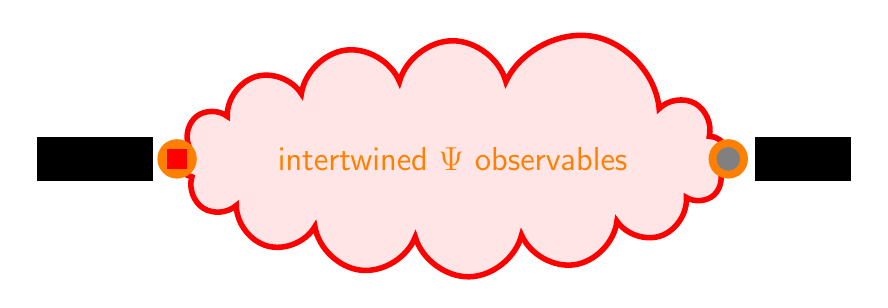
\begin{tikzpicture}  [scale=0.25,font=\large\sffamily]

\newdimen\ms
\ms=0.1cm


\tikzstyle{s1}=[color=red,rectangle,inner sep=3.5]
\tikzstyle{c3}=[circle,inner sep={\ms/8},minimum size=5*\ms]
\tikzstyle{c2}=[circle,inner sep={\ms/8},minimum size=3*\ms]
\tikzstyle{c1}=[circle,inner sep={\ms/8},minimum size=2*\ms]

\tikzstyle{every path}=[line width=2pt]

% Radius of regular polygons
\newdimen\R
\R=14cm     % outer circle

%\r= { \R * sqrt(3) }     % inner circle
%\newdimen\r
%\r=    {\R * sqrt(3)/2}       % inner circle

%\newdimen\K
%\K=3cm

% Define positions of all observables
\path
  ({180 + 0 * 360 /2}:\R      ) coordinate(1)
  ({180 + 1 * 360 /2}:\R   ) coordinate(2)
;

% draw contexts

%\draw [draw=violet!30]  (0,0) circle[radius=\R ] node[above right] { };

\draw [color=orange] (1) -- (2);

\node[cloud, cloud puffs=15.7, cloud ignores aspect, minimum width=5cm, minimum height=3cm, align=center, draw] (cloud) [color=red,fill=red!10]  at (0cm, 0cm) {{\color{orange}\vspace{1cm}  intertwined $\Psi$~observables \vspace{1cm} }};


%
%%
%% draw atoms
%%
%

\draw (1) coordinate[c3,fill=orange];   %
\draw (1) coordinate[s1,fill=red,label=180:\colorbox{black}{\Large \bf Alice}];  %

\draw (2) coordinate[c3,fill=orange];   %
\draw (2) coordinate[c2,fill=gray,label=right:{\Large  \colorbox{black}{\bf Bob}}];  %
%
\end{tikzpicture}
\end{center}


 }

 \frame{
 \frametitle{\color{orange!100}How is $\vert {\bf Bob}\rangle$ given $\vert {\bf Alice}\rangle$? True? False? Whatever? None?
 }
\setlength\tabcolsep{0.5pt} % default value: 6pt
\begin{center}
\begin{tabular}{cc}
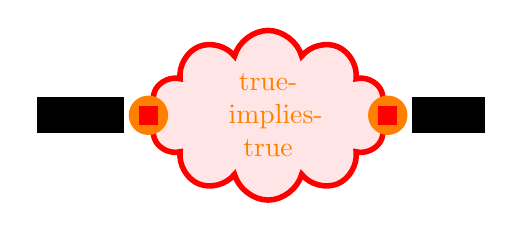
\begin{tikzpicture}  [scale=0.08]

\newdimen\ms
\ms=0.1cm


\tikzstyle{s1}=[color=red,rectangle,inner sep=3.5]
\tikzstyle{c3}=[circle,inner sep={\ms/8},minimum size=5*\ms]
\tikzstyle{c2}=[circle,inner sep={\ms/8},minimum size=3*\ms]
\tikzstyle{c1}=[circle,inner sep={\ms/8},minimum size=2*\ms]

\tikzstyle{every path}=[line width=2pt]

% Radius of regular polygons
\newdimen\R
\R=19cm     % outer circle

%\r= { \R * sqrt(3) }     % inner circle
%\newdimen\r
%\r=    {\R * sqrt(3)/2}       % inner circle

%\newdimen\K
%\K=3cm

% Define positions of all observables
\path
  ({180 + 0 * 360 /2}:\R      ) coordinate(1)
  ({180 + 1 * 360 /2}:\R   ) coordinate(2)
;

% draw contexts

%\draw [draw=violet!30]  (0,0) circle[radius=\R ] node[above right] { };

\draw [color=orange] (1) -- (2);

\node[cloud, cloud puffs=10, cloud ignores aspect, minimum width=3cm, minimum height=2cm, align=center, draw, text width=1cm] (cloud) [color=red,fill=red!10]  at (0cm, 0cm) {{\color{orange}true-implies-true}};


%
%%
%% draw atoms
%%
%

\draw (1) coordinate[c3,fill=orange];   %
\draw (1) coordinate[s1,fill=red,label=180:\colorbox{black}{\bf Alice}];  %

\draw (2) coordinate[c3,fill=orange];   %
\draw (2) coordinate[s1,fill=red,label=right:{\colorbox{black}{\bf Bob}}];  %
%
\end{tikzpicture}
&
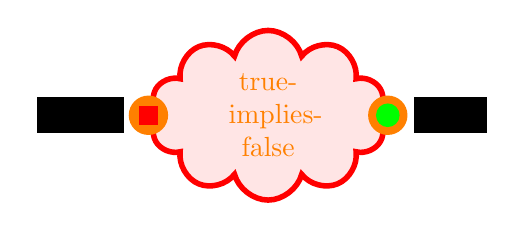
\begin{tikzpicture}  [scale=0.08]

\newdimen\ms
\ms=0.1cm


\tikzstyle{s1}=[color=red,rectangle,inner sep=3.5]
\tikzstyle{c3}=[circle,inner sep={\ms/8},minimum size=5*\ms]
\tikzstyle{c2}=[circle,inner sep={\ms/8},minimum size=3*\ms]
\tikzstyle{c1}=[circle,inner sep={\ms/8},minimum size=2*\ms]

\tikzstyle{every path}=[line width=2pt]

% Radius of regular polygons
\newdimen\R
\R=19cm     % outer circle

%\r= { \R * sqrt(3) }     % inner circle
%\newdimen\r
%\r=    {\R * sqrt(3)/2}       % inner circle

%\newdimen\K
%\K=3cm

% Define positions of all observables
\path
  ({180 + 0 * 360 /2}:\R      ) coordinate(1)
  ({180 + 1 * 360 /2}:\R   ) coordinate(2)
;

% draw contexts

%\draw [draw=violet!30]  (0,0) circle[radius=\R ] node[above right] { };

\draw [color=orange] (1) -- (2);

\node[cloud, cloud puffs=10, cloud ignores aspect, minimum width=3cm, minimum height=2cm, align=center, draw, text width=1cm] (cloud) [color=red,fill=red!10]  at (0cm, 0cm) {{\color{orange}true-implies-false}};


%
%%
%% draw atoms
%%
%

\draw (1) coordinate[c3,fill=orange];   %
\draw (1) coordinate[s1,fill=red,label=180:\colorbox{black}{\bf Alice}];  %

\draw (2) coordinate[c3,fill=orange];   %
\draw (2) coordinate[c2,fill=green,label=right:{\colorbox{black}{\bf Bob}}];  %
%
\end{tikzpicture}
\\
$\quad$
\\
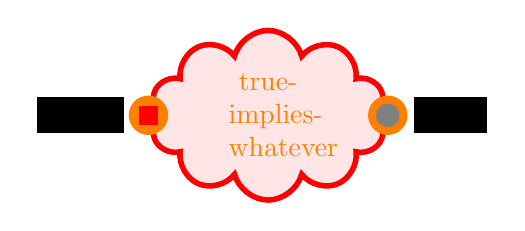
\begin{tikzpicture}  [scale=0.08]

\newdimen\ms
\ms=0.1cm


\tikzstyle{s1}=[color=red,rectangle,inner sep=3.5]
\tikzstyle{c3}=[circle,inner sep={\ms/8},minimum size=5*\ms]
\tikzstyle{c2}=[circle,inner sep={\ms/8},minimum size=3*\ms]
\tikzstyle{c1}=[circle,inner sep={\ms/8},minimum size=2*\ms]

\tikzstyle{every path}=[line width=2pt]

% Radius of regular polygons
\newdimen\R
\R=19cm     % outer circle

%\r= { \R * sqrt(3) }     % inner circle
%\newdimen\r
%\r=    {\R * sqrt(3)/2}       % inner circle

%\newdimen\K
%\K=3cm

% Define positions of all observables
\path
  ({180 + 0 * 360 /2}:\R      ) coordinate(1)
  ({180 + 1 * 360 /2}:\R   ) coordinate(2)
;

% draw contexts

%\draw [draw=violet!30]  (0,0) circle[radius=\R ] node[above right] { };

\draw [color=orange] (1) -- (2);

\node[cloud, cloud puffs=10, cloud ignores aspect, minimum width=3cm, minimum height=2cm, align=center, draw, text width=1cm] (cloud) [color=red,fill=red!10]  at (0cm, 0cm) {{\color{orange}true-implies-whatever}};


%
%%
%% draw atoms
%%
%

\draw (1) coordinate[c3,fill=orange];   %
\draw (1) coordinate[s1,fill=red,label=180:\colorbox{black}{\bf Alice}];  %

\draw (2) coordinate[c3,fill=orange];   %
\draw (2) coordinate[c2,fill=gray,label=right:{\colorbox{black}{\bf Bob}}];  %
%
\end{tikzpicture}
&
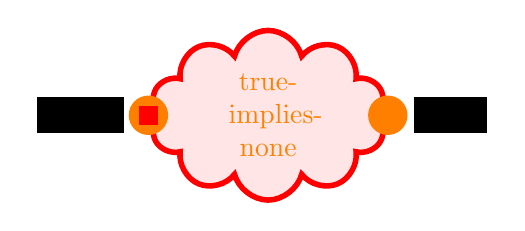
\begin{tikzpicture}  [scale=0.08]

\newdimen\ms
\ms=0.1cm


\tikzstyle{s1}=[color=red,rectangle,inner sep=3.5]
\tikzstyle{c3}=[circle,inner sep={\ms/8},minimum size=5*\ms]
\tikzstyle{c2}=[circle,inner sep={\ms/8},minimum size=3*\ms]
\tikzstyle{c1}=[circle,inner sep={\ms/8},minimum size=2*\ms]

\tikzstyle{every path}=[line width=2pt]

% Radius of regular polygons
\newdimen\R
\R=19cm     % outer circle

%\r= { \R * sqrt(3) }     % inner circle
%\newdimen\r
%\r=    {\R * sqrt(3)/2}       % inner circle

%\newdimen\K
%\K=3cm

% Define positions of all observables
\path
  ({180 + 0 * 360 /2}:\R      ) coordinate(1)
  ({180 + 1 * 360 /2}:\R   ) coordinate(2)
;

% draw contexts

%\draw [draw=violet!30]  (0,0) circle[radius=\R ] node[above right] { };

\draw [color=orange] (1) -- (2);

\node[cloud, cloud puffs=10, cloud ignores aspect, minimum width=3cm, minimum height=2cm, align=center, draw, text width=1cm] (cloud) [color=red,fill=red!10]  at (0cm, 0cm) {{\color{orange}true-implies-none}};


%
%%
%% draw atoms
%%
%

\draw (1) coordinate[c3,fill=orange];   %
\draw (1) coordinate[s1,fill=red,label=180:\colorbox{black}{\bf Alice}];  %

\draw (2) coordinate[c3,fill=orange];   %
\draw (2) coordinate[c2,fill=orange,label=right:{\colorbox{black}{\bf Bob}}];  %
%
\end{tikzpicture}
\end{tabular}
\end{center}
%\begin{flushleft}
%{\small  Ad�n Cabello, Jos� R. Portillo, Alberto Sol�s, KS, Minimal true-implies-false and true-implies-true sets of propositions..., arXiv:1805.00796}
%\end{flushleft}


 }


\begin{frame}[fragile]{True (1) implies whatever (quantum 50:50)}

\begin{center}
\begin{tikzpicture}  [scale=0.30]

\newdimen\ms
\ms=0.05cm

\tikzstyle{every path}=[line width=2pt]

\tikzstyle{s1}=[color=red,rectangle,inner sep=3.5]
\tikzstyle{c3}=[circle,inner sep={\ms/8},minimum size=5*\ms]
\tikzstyle{c2}=[circle,inner sep={\ms/8},minimum size=3*\ms]
\tikzstyle{c1}=[circle,inner sep={\ms/8},minimum size=2*\ms]

% Radius of regular polygons
\newdimen\R
\R=6cm     % outer circle

%\r= { \R * sqrt(3) }     % inner circle
%\newdimen\r
%\r=    {\R * sqrt(3)/2}       % inner circle

%\newdimen\K
%\K=3cm

% Define positions of all observables
\path
  (0,6 ) coordinate(1)
  (3,3    ) coordinate(2)
  (6,0 ) coordinate(3)
  (9,3) coordinate(4)
  (12,6  ) coordinate(5)
;

% draw contexts

\draw [color=yellow] (1) -- (2) -- (3);
\draw [color=blue] (3) -- (4) -- (5);


%
%%
%% draw atoms
%%
%
\draw (1) coordinate[s1,fill=red,label={above:$\vert {\bf Alice} \rangle = \begin{pmatrix}1,0,0\end{pmatrix}$}];   %
%
\draw (2) coordinate[c3,fill=yellow,label={left: $\frac{1}{\sqrt{2}}\begin{pmatrix}0,1,1\end{pmatrix}$}];    %
%
\draw (3) coordinate[c3,fill=blue,label={below: $\frac{1}{\sqrt{2}}\begin{pmatrix}0,1,-1\end{pmatrix}$}]; %
\draw (3) coordinate[c2,fill=yellow];  %
%
\draw (4) coordinate[c3,fill=blue,label={right: $\begin{pmatrix} -\frac{1}{\sqrt{2}},\frac{1}{2},\frac{1}{2}\end{pmatrix}$}];  %
%
\draw (5) coordinate[c3,fill=gray,label={above: $\vert {\bf Bob} \rangle = \begin{pmatrix}   \frac{1}{\sqrt{2}},\frac{1}{2},\frac{1}{2} \end{pmatrix}$}];  %
%
%

\end{tikzpicture}
\end{center}

\end{frame}


\begin{frame}[fragile]{True (1) implies false (0)}

\newif\iflabel \labelfalse
\begin{center}
\begin{tikzpicture}  [scale=0.20, rotate=117]

        \tikzstyle{every path}=[line width=1.5pt]
        \tikzstyle{c1}=[color=green,circle,inner sep=2.5]
        \tikzstyle{s1}=[color=red,rectangle,inner sep=3.5]
        \tikzstyle{l1}=[draw=none,circle,minimum size=4]

        % Define positions of all observables

\draw [color=orange]   (4,0) coordinate[c1,fill,label=0:{\color{white}\normalsize $\vert {\bf Bob} \rangle = \begin{pmatrix}   \frac{1}{\sqrt{2}},\frac{1}{2},\frac{1}{2} \end{pmatrix}$}] (b) -- (13,0)     coordinate[c1,fill,label=270:{\iflabel \tiny $P_2$\fi}] (2) -- (22,0)  coordinate[s1,fill,label=315:{\iflabel \tiny $P_3$\fi}] (3);
\draw [color=blue,   ] (3) -- (26,12)  coordinate[c1,fill,pos=0.8,label=0:{\iflabel \tiny $P_{21}$\fi}] (21) coordinate[c1,fill,label=0:{\iflabel \tiny $P_{23}$\fi}] (23);
\draw [color=black] (23) -- (22,18.5) coordinate[c1,fill,pos=0.4,color=black,label=0:{\iflabel \tiny $P_{29}$\fi}] (29) coordinate[c1,fill,label=45:{\iflabel \tiny $P_5$\fi}] (5);
\draw [color=magenta,] (5)-- (13,18.5)coordinate[s1,fill,label=180:{\color{white}\normalsize $\vert {\bf Alice} \rangle = \begin{pmatrix}1,0,0\end{pmatrix}$}] (a) -- (4,18.5)  coordinate[c1,fill,label=135:{\iflabel \tiny $P_4$\fi}] (4);
\draw [color=CadetBlue, ] (4) -- (0,12)   coordinate[c1,fill,pos=0.6,label=180:{\iflabel \tiny $P_{10}$\fi}] (10) coordinate[s1,fill,label=180:{\iflabel \tiny $P_7$\fi}] (7);
\draw [color=brown,  ](7) -- (b)       coordinate[c1,fill,pos=0.2,label=180:{\iflabel \tiny $P_6$\fi}] (6);

        \draw [color=gray] (a) -- (2) coordinate[c1,fill,pos=0.5,label=315:{\iflabel \tiny $P_1$\fi}] (1);

        \draw [color=violet] (5) -- (22,6) coordinate[s1,fill,pos=0.4,label=0:{\iflabel \tiny $P_{11}$\fi}] (11) coordinate[c1,fill,label=0:{\iflabel \tiny $P_9$\fi}] (9);

\draw [color=Apricot] (9) -- (b) coordinate[s1,fill,pos=0.3,label=280:{\iflabel \tiny $P_8$\fi}] (8);

\draw [color=TealBlue] (4) -- (4,6) coordinate[s1,fill,pos=0.4,label=180:{\iflabel \tiny $P_{28}$\fi}] (28) coordinate[c1,fill,label=180:{\iflabel \tiny $P_{22}$\fi}] (22);
\draw [color=YellowGreen] (22) -- (3) coordinate[c1,fill,pos=0.2,label=260:{\iflabel \tiny $P_{19}$\fi}] (19);

        \coordinate (25) at ([xshift=-4cm]1);
        \coordinate (27) at ([xshift=4cm]1);

\draw [color=MidnightBlue]  (22) -- (25) coordinate[c1,fill,pos=0.5,label=115:{\iflabel \tiny $P_{24}$\fi}] (24) coordinate[s1,fill,label=270:{\iflabel \tiny $P_{25}$\fi}] (25);
\draw [color=Mulberry] (25) -- (9) coordinate[c1,fill,pos=0.8,label=90:{\iflabel \tiny $P_{35}$\fi}] (35);

\draw [color=BrickRed]  (7) -- (27) coordinate[c1,fill,pos=0.5,label=90:{\iflabel \tiny $P_{34}$\fi}] (34) coordinate[c1,fill,label=90:{\iflabel \tiny $P_{27}$\fi}] (27);
\draw [color=Emerald] (27) -- (23) coordinate[s1,fill,pos=0.25,label=270:{\iflabel \tiny $P_{26}$\fi}] (26);

\draw [color=BlueGreen]  (10) -- (15.5,17.5) coordinate[c1,fill,pos=0.5,label=90:{\iflabel \tiny $P_{12}$\fi}] (12) coordinate[s1,fill,label=15:{\iflabel \tiny $P_{13}$\fi}] (13);
%\draw [color=Tan] (13) -- (29) coordinate[c1,fill,pos=0.4,label=90:{\iflabel \tiny $P_{31}$\fi}] (31);

\draw [color=RawSienna]  (28) -- (10.5,15) coordinate[c1,fill,pos=0.5,label=90:{\iflabel \tiny $P_{30}$\fi}] (30) coordinate[c1,fill,label=90:{\iflabel \tiny $P_{15}$\fi}] (15);
\draw [color=SpringGreen] (15) -- (11) coordinate[c1,fill,pos=0.6,label=90:{\iflabel \tiny $P_{14}$\fi}] (14);

\draw [color=Salmon]  (15) -- (1) coordinate[s1,fill,pos=0.2,label=15:{\iflabel \tiny $P_{17}$\fi}] (17);
\draw [color=Fuchsia] (1)-- (13) coordinate[c1,fill,pos=0.3,label=0:{\iflabel \tiny $P_{16}$\fi}] (16);

\draw [color=CornflowerBlue]  (19) -- (16) coordinate[s1,fill,pos=0.3,label=180:{\iflabel \tiny $P_{18}$\fi}] (18);
\draw [color=pink] (16) -- (8) coordinate[c1,fill,pos=0.7,label=180:{\iflabel \tiny $P_{32}$\fi}] (32);

\draw [color=PineGreen]  (6) -- (17) coordinate[c1,fill,pos=0.7,label=90:{\iflabel \tiny $P_{33}$\fi}] (33);
\draw [color=DarkOrchid] (17) -- (21) coordinate[c1,fill,pos=0.4,label=90:{\iflabel \tiny $P_{20}$\fi}] (20);

\draw [color=white] (25)  -- (1) -- (27);

%\coordinate (ContextLabel) at ([shift=({-2cm,-3mm})]1);
%\draw (ContextLabel) coordinate[l1,label=90:{\iflabel \tiny $C_{26}$\fi}];

\end{tikzpicture}
\end{center}
\end{frame}

\begin{frame}[fragile]{True (1) implies true (1)}

\newif\iflabel
\labelfalse
\begin{center}
\begin{tikzpicture}  [scale=0.20, rotate=117]

        \tikzstyle{every path}=[line width=1.5pt]
        \tikzstyle{c1}=[color=green,circle,inner sep=2.5]
        \tikzstyle{s1}=[color=red,rectangle,inner sep=3.5]
        \tikzstyle{l1}=[draw=none,circle,minimum size=4]

        % Define positions of all observables

\draw [color=orange]   (4,0) coordinate[s1,fill,label=0:{\color{white}\normalsize $\vert {\bf Bob} \rangle = \begin{pmatrix}   \frac{1}{\sqrt{2}},\frac{1}{2},\frac{1}{2} \end{pmatrix}$}] (b) -- (13,0)     coordinate[c1,fill,label=270:{\iflabel \tiny $P_2$\fi}] (2) -- (22,0)  coordinate[c1,fill,label=315:{\iflabel \tiny $P_3$\fi}] (3);
\draw [color=blue,   ] (3) -- (26,12)  coordinate[c1,fill,pos=0.8,label=0:{\iflabel \tiny $P_{21}$\fi}] (21) coordinate[s1,fill,label=0:{\iflabel \tiny $P_{23}$\fi}] (23);
\draw [color=green] (23) -- (22,18.5) coordinate[c1,fill,pos=0.4,label=0:{\iflabel \tiny $P_{29}$\fi}] (29) coordinate[c1,fill,label=45:{\iflabel \tiny $P_5$\fi}] (5);
\draw [color=magenta,] (5)-- (13,18.5)coordinate[s1,fill,label=180:{\color{white}\normalsize $\vert {\bf Alice} \rangle = \begin{pmatrix}1,0,0\end{pmatrix}$}] (a) -- (4,18.5)  coordinate[c1,fill,label=135:{\iflabel \tiny $P_4$\fi}] (4);
\draw [color=black] (4) -- (0,12)   coordinate[c1,color=black,fill,pos=0.6,label=180:{\iflabel \tiny $P_{10}$\fi}] (10) coordinate[c1,fill,label=180:{\iflabel \tiny $P_7$\fi}] (7);
\draw [color=brown,  ] (7) -- (b)      coordinate[c1,fill,pos=0.2,label=180:{\iflabel \tiny $P_6$\fi}] (6);

        \draw [color=gray] (a) -- (2) coordinate[c1,fill,pos=0.5,label=315:{\iflabel \tiny $P_1$\fi}] (1);

        \draw [color=violet] (5) -- (22,6) coordinate[s1,fill,pos=0.4,label=0:{\iflabel \tiny $P_{11}$\fi}] (11) coordinate[c1,fill,label=0:{\iflabel \tiny $P_9$\fi}] (9);

\draw [color=Apricot] (9) -- (b) coordinate[c1,fill,pos=0.3,label=280:{\iflabel \tiny $P_8$\fi}] (8);

\draw [color=TealBlue] (4) -- (4,6) coordinate[s1,fill,pos=0.4,label=180:{\iflabel \tiny $P_{28}$\fi}] (28) coordinate[c1,fill,label=180:{\iflabel \tiny $P_{22}$\fi}] (22);
\draw [color=YellowGreen] (22) -- (3) coordinate[s1,fill,pos=0.2,label=260:{\iflabel \tiny $P_{19}$\fi}] (19);

        \coordinate (25) at ([xshift=-4cm]1);
        \coordinate (27) at ([xshift=4cm]1);

\draw [color=MidnightBlue]  (22) -- (25) coordinate[c1,fill,pos=0.5,label=115:{\iflabel \tiny $P_{24}$\fi}] (24) coordinate[s1,fill,label=270:{\iflabel \tiny $P_{25}$\fi}] (25);
\draw [color=Mulberry] (25) -- (9) coordinate[s1,fill,pos=0.8,label=90:{\iflabel \tiny $P_{35}$\fi}] (35);

\draw [color=BrickRed]  (7) -- (27) coordinate[s1,fill,pos=0.5,label=90:{\iflabel \tiny $P_{34}$\fi}] (34) coordinate[c1,fill,label=90:{\iflabel \tiny $P_{27}$\fi}] (27);
\draw [color=Emerald] (27) -- (23) coordinate[c1,fill,pos=0.25,label=270:{\iflabel \tiny $P_{26}$\fi}] (26);

\draw [color=black]  (10) -- (15.5,17.5) coordinate[c1,color=black,fill,pos=0.5,label=90:{\iflabel \tiny $P_{12}$\fi}] (12) coordinate[s1,fill,label=15:{\iflabel \tiny $P_{13}$\fi}] (13);
\draw [color=Tan] (13) -- (29) coordinate[c1,fill,pos=0.4,label=90:{\iflabel \tiny $P_{31}$\fi}] (31);

\draw [color=RawSienna]  (28) -- (10.5,15) coordinate[c1,fill,pos=0.5,label=90:{\iflabel \tiny $P_{30}$\fi}] (30) coordinate[c1,fill,label=90:{\iflabel \tiny $P_{15}$\fi}] (15);
\draw [color=SpringGreen] (15) -- (11) coordinate[c1,fill,pos=0.6,label=90:{\iflabel \tiny $P_{14}$\fi}] (14);

\draw [color=Salmon]  (15) -- (1) coordinate[s1,fill,pos=0.2,label=15:{\iflabel \tiny $P_{17}$\fi}] (17);
\draw [color=Fuchsia] (1)-- (13) coordinate[c1,fill,pos=0.3,label=0:{\iflabel \tiny $P_{16}$\fi}] (16);

\draw [color=CornflowerBlue]  (19) -- (16) coordinate[c1,fill,pos=0.3,label=180:{\iflabel \tiny $P_{18}$\fi}] (18);
\draw [color=pink] (16) -- (8) coordinate[s1,fill,pos=0.7,label=180:{\iflabel \tiny $P_{32}$\fi}] (32);

\draw [color=PineGreen]  (6) -- (17) coordinate[c1,fill,pos=0.7,label=90:{\iflabel \tiny $P_{33}$\fi}] (33);
\draw [color=DarkOrchid] (17) -- (21) coordinate[c1,fill,pos=0.4,label=90:{\iflabel \tiny $P_{20}$\fi}] (20);

\draw [color=white] (25) -- (1) -- (27);

        \coordinate (ContextLabel) at ([shift=({-2cm,-3mm})]1);
        \draw (ContextLabel) coordinate[l1,label=90:{\iflabel \tiny $C_{26}$\fi}];

        \end{tikzpicture}
\end{center}
\end{frame}

\begin{frame}[fragile]{True (1) implies value indefinite (Abbott, Calude, KS 2015)}

\newif\iflabel \labelfalse
\begin{center}
\begin{tikzpicture}  [scale=0.20, rotate=117]
\labelfalse
        \tikzstyle{every path}=[line width=1.5pt]
%\tikzstyle{c1}=[circle,fill,inner sep=4]
%\tikzstyle{c2}=[circle,fill,inner sep=2.7]
%\tikzstyle{c3}=[circle,fill,inner sep=1]
        \tikzstyle{c1}=[circle,fill,inner sep=3]
        \tikzstyle{c2}=[circle,fill,inner sep=2]
        \tikzstyle{c3}=[circle,fill,inner sep=1]
        \tikzstyle{s1}=[color=red,rectangle,minimum size=8,inner sep=6]
        \tikzstyle{d1}=[draw=none,circle,minimum size=4]
        \tikzstyle{e1}=[color=gray,rectangle,minimum size=8,inner sep=6]

        % Define positions of all observables



\draw [color=orange]  (4,0)  coordinate[c1,fill,label=0:{\color{white}\normalsize $\vert {\bf Bob} \rangle = \begin{pmatrix}   \frac{1}{\sqrt{2}},\frac{1}{2},\frac{1}{2} \end{pmatrix}$}] (b) -- (13,0)    coordinate[c1,fill,label={[label distance=-1]270:{\iflabel \footnotesize \color{white}  $2$\fi}}] (2) -- (22,0)  coordinate[c1,fill,label={[label distance=-1]315:{\iflabel \footnotesize \color{white}  $3$\fi}}] (3);
\draw [color=blue] (3) -- (26,12)  coordinate[c1,fill,pos=0.8,label={[label distance=-1]0:{\iflabel \footnotesize \color{white}  ${21}$\fi}}] (21) coordinate[c1,fill,label={[label distance=-3]0:{\iflabel \footnotesize \color{white}  ${23}$\fi}}] (23);
\draw [color=green] (23) -- (22,18.5) coordinate[c1,fill,pos=0.4,label={[label distance=-1]0:{\iflabel \footnotesize \color{white}  ${29}$\fi}}] (29) coordinate[c1,fill,label={[label distance=-1]45:{\iflabel \footnotesize \color{white}  $5$\fi}}] (5);
\draw [color=magenta] (5)-- (13,18.5)coordinate[c1,fill,label=180:{\color{white}\normalsize $\vert {\bf Alice} \rangle = \begin{pmatrix}1,0,0\end{pmatrix}$}] (a) -- (4,18.5)  coordinate[c1,fill,label={[label distance=-1]135:{\iflabel \footnotesize \color{white}  $4$\fi}}] (4);
\draw [color=CadetBlue] (4) -- (0,12)   coordinate[c1,fill,pos=0.6,label={[label distance=-1]180:{\iflabel \footnotesize \color{white}  ${10}$\fi}}] (10)  coordinate[c1,fill,label={[label distance=-1]180:{\iflabel \footnotesize \color{white}  $7$\fi}}] (7);
\draw [color=brown] (7) -- (b)      coordinate[c1,fill,pos=0.2,label={[label distance=-1]180:{\iflabel \footnotesize \color{white}  $6$\fi}}] (6);






        \draw [color=gray] (a) -- (2) coordinate[c1,fill,pos=0.52,label={[label distance=-1, yshift=2]357.5:{\iflabel \footnotesize \color{white}  $1$\fi}}] (1);

        \draw [color=violet] (5) -- (22,6) coordinate[c1,fill,pos=0.4,label={[label distance=-1]0:{\iflabel \footnotesize \color{white}  ${11}$\fi}}] (11) coordinate[c1,fill,label={[label distance=-1]0:{\iflabel \footnotesize \color{white}  $9$\fi}}] (9);

\draw [color=Apricot] (9) -- (b) coordinate[c1,fill,pos=0.3,label={[label distance=-1]280:{\iflabel \footnotesize \color{white}  $8$\fi}}] (8);

\draw [color=TealBlue] (4) -- (4,6) coordinate[c1,fill,pos=0.4,label={[label distance=-1]180:{\iflabel \footnotesize \color{white}  ${28}$\fi}}] (28) coordinate[c1,fill,label={[label distance=-3]180:{\iflabel \footnotesize \color{white}  ${22}$\fi}}] (22);
\draw [color=YellowGreen] (22) -- (3) coordinate[c1,fill,pos=0.2,label={[label distance=-1]260:{\iflabel \footnotesize \color{white}  ${19}$\fi}}] (19);

        \coordinate (25) at ([xshift=-4cm]1);
        \coordinate (27) at ([xshift=4cm]1);

\draw [color=MidnightBlue]  (22) -- (25) coordinate[c1,fill,pos=0.5,label={[label distance=-1]180:{\iflabel \footnotesize \color{white}  ${24}$\fi}}] (24) coordinate[c1,fill,label={[label distance=-1]180:{\iflabel \footnotesize \color{white}  ${25}$\fi}}] (25);
\draw [color=Mulberry] (25) -- (9) coordinate[c1,fill,pos=0.8,label={[label distance=-1]90:{\iflabel \footnotesize \color{white}  ${35}$\fi}}] (35);

\draw [color=BrickRed]  (7) -- (27) coordinate[c1,fill,pos=0.5,label={[label distance=-3]90:{\iflabel \footnotesize \color{white}  ${34}$\fi}}] (34) coordinate[c1,fill,label={[label distance=-1]90:{\iflabel \footnotesize \color{white}  ${27}$\fi}}] (27);
\draw [color=Emerald] (27) -- (23) coordinate[c1,fill,pos=0.25,label={[label distance=-1]320:{\iflabel \footnotesize \color{white}  ${26}$\fi}}] (26);

\draw [color=BlueGreen]  (10) -- (15.5,17.5) coordinate[c1,fill,pos=0.5,label={[label distance=-1]90:{\iflabel \footnotesize \color{white}  ${12}$\fi}}] (12) coordinate[c1,fill,label={[label distance=-1,xshift=5]270:{\iflabel \footnotesize \color{white}  ${13}$\fi}}] (13);
\draw [color=Tan] (13) -- (29) coordinate[c1,fill,pos=0.4,label={[label distance=-1]90:{\iflabel \footnotesize \color{white}  ${31}$\fi}}] (31);

\draw [color=RawSienna]  (28) -- (10.5,15) coordinate[c1,fill,pos=0.5,label={[label distance=-3, yshift=-3]160:{\iflabel \footnotesize \color{white}  ${30}$\fi}}] (30) coordinate[c1,fill,label={[label distance=-5]45:{\iflabel \footnotesize \color{white}  ${15}$\fi}}] (15);
\draw [color=SpringGreen] (15) -- (11) coordinate[c1,fill,pos=0.6,label={[label distance=-1]90:{\iflabel \footnotesize \color{white}  ${14}$\fi}}] (14);

\draw [color=Salmon]  (15) -- (1) coordinate[c1,fill,pos=0.2,label={[label distance=-1, yshift=2]180:{\iflabel \footnotesize \color{white}  ${17}$\fi}}] (17);
\draw [color=Fuchsia] (1)-- (13) coordinate[c1,fill,pos=0.3,label={[label distance=-1]0:{\iflabel \footnotesize \color{white}  ${16}$\fi}}] (16);

\draw [color=CornflowerBlue]  (19) -- (16) coordinate[c1,fill,pos=0.3,label={[label distance=-1]180:{\iflabel \footnotesize \color{white}  ${18}$\fi}}] (18);
\draw [color=pink] (16) -- (8) coordinate[c1,fill,pos=0.7,label={[label distance=-1]180:{\iflabel \footnotesize \color{white}  ${32}$\fi}}] (32);

\draw [color=PineGreen]  (6) -- (17) coordinate[c1,fill,pos=0.7,label={[label distance=-1, yshift=2]180:{\iflabel \footnotesize \color{white}  ${33}$\fi}}] (33);
\draw [color=DarkOrchid] (17) -- (21) coordinate[c1,fill,pos=0.4,label={[label distance=-3]20:{\iflabel \footnotesize \color{white}  ${20}$\fi}}] (20);

\draw [color=white] (25) -- (1) -- (27);




\draw (a) coordinate[c2,fill=gray];

\draw (b) coordinate[c2,fill=brown];
\draw (b) coordinate[c3,fill=Apricot];

\draw (4) coordinate[c2,fill=CadetBlue];
\draw (4) coordinate[c3,fill=TealBlue];

\draw (5) coordinate[c2,fill=magenta];
\draw (5) coordinate[c3,fill=violet];

\draw (7) coordinate[c2,BrickRed];
\draw (7) coordinate[c3,fill=brown];

\draw (23) coordinate[c2,fill=green];
\draw (23) coordinate[c3,fill=Emerald];

\draw (29) coordinate[c2,fill=Tan];

\draw (21) coordinate[c2,fill=DarkOrchid];

\draw (3) coordinate[c2,fill=blue];
\draw (3) coordinate[c3,fill=YellowGreen];

\draw (11) coordinate[c2,fill=SpringGreen];

\draw (9) coordinate[c2,fill=Apricot];
\draw (9) coordinate[c3,fill=Mulberry];

\draw (27) coordinate[c2,fill=Emerald];
\draw (27) coordinate[c3,fill=black];

\draw (13) coordinate[c2,fill=Tan];
\draw (13) coordinate[c3,fill=Fuchsia];

\draw (7) coordinate[c2,BrickRed];
\draw (7) coordinate[c3,fill=brown];

\draw (8) coordinate[c2,fill=pink];

\draw (19) coordinate[c2,fill=CornflowerBlue];

\draw (16) coordinate[c2,fill=CornflowerBlue];
\draw (16) coordinate[c3,fill=pink];

\draw (1) coordinate[c2,fill=Salmon];
\draw (1) coordinate[c3,fill=Fuchsia];

\draw (17) coordinate[c2,fill=PineGreen];
\draw (17) coordinate[c3,fill=DarkOrchid];

\draw (15) coordinate[c2,fill=SpringGreen];
\draw (15) coordinate[c3,fill=Salmon];

\draw (25) coordinate[c2,fill=Mulberry];
\draw (25) coordinate[c3,fill=black];


\draw (22) coordinate[c2,fill=YellowGreen];
\draw (22) coordinate[c3,fill=MidnightBlue];

\draw (28) coordinate[c2,fill=RawSienna];

\draw (10) coordinate[c2,fill=BlueGreen];

\draw (6) coordinate[c2,fill=PineGreen];


\draw (2) coordinate[c2,fill=gray];

\end{tikzpicture}
 \end{center}
\end{frame}


\begin{frame}[fragile]{Strategies to obtain  value indefiniteness/partiality}

The scheme of the construction \& proof of partiality of value assignments is as follows:
\begin{itemize}
\item[(i)]
Find a logic (collection of intertwined contexts of observables) exhibiting a true-implies-false  property on the two atoms ${\bf a}$ and ${\bf b}$.
\item[(ii)]
Find another logic exhibiting a true-implies-true property on the same two atoms ${\bf a}$ and ${\bf b}$.
\item[(iii)]
Then join (paste) these logics into a larger logic, which, given ${\bf a}$,
neither allows ${\bf b}$ to be true nor false. Consequently  ${\bf b}$ must be value indefinite.
\end{itemize}

\end{frame}

\begin{frame}[fragile]{Extensions of value indefiniteness/partiality}

Partiality/value indefiniteness can be extended to {\color{red}any}
vector ${\bf b}$ non-collinear and non-orthogonal to ${\bf a}$:
Alastair A. Abbott and Cristian S. Calude and KS,
``A variant of the {K}ochen-{S}pecker theorem localising value indefiniteness'',
Journal of Mathematical Physics, {\bf 56}(10), 102201(1-17),2015;  https://doi.org/10.1063/1.4931658
\begin{center}\color{orange}
$\widetilde{\qquad \qquad }$
$\widetilde{\qquad \qquad}$
$\widetilde{\qquad \qquad }$
\end{center}
For a (in some respects weaker) statement relative to global truth assignments, see
Itamar Pitowsky's ``Infinite and finite {G}leason's theorems and the logic of indeterminacy'',
Journal of Mathematical Physics {\bf 39}(1),218-228, 1998; https://doi.org/10.1063/1.532334

\end{frame}



\begin{frame}[fragile]{History of contextual sets \& elational properties realizable by two-point quantum clouds}

{\tiny
\begin{tabular}{lll}
 \hline\hline
if ${\bf a}$ is true classical value assignments  & anectodal, historic & reference to utility\\
&quantum realisation & or relational properties \\
\hline\hline
imply ${\bf b}$ is independent (arbitrary) & firefly logic $L_{12}$\\
&eg, Cohen, 1989[pp.~21,~22]&  \\
 \hline
imply ${\bf b}$ false (TIFS)  & Specker bug logic& Stairs, 1983 [p.~588-589],\\
&KS, 1965 [Fig.~1, p.~182] &   Cabello et al, 1995 $\ldots$ 2018\\
 \hline
imply ${\bf b}$ true (TITS)  & extended Specker bug&  KS, 1967 [$\Gamma_1$, p.~68],\\
& logic &  Clifton, 1993 [Sects.~II,III, Fig.~1],
\\
&&Belinfante, 73 [Fig.~C.l. p.~67],\\
&&   Pitowsky, 1982 [p.~394],\\
&& Hardy, 1992, 1993, 1997, \\
&&Cabello et al, 1995 $\ldots$ 2018\\
 \hline
iff ${\bf b}$ true  (nonseparability) & combo of intertwined&  KS, 1967 [$\Gamma_3$, p.~70]\\
& Specker bugs \\
 \hline
imply value indefiniteness of ${\bf b}$  & depending on types &  Pitowsky, 1998, \\
& of value assignments & Abbott et al, 2012 $\ldots$ 2015\\
 \hline\hline
\end{tabular}
}

\end{frame}

 \frame{
 \frametitle{\color{orange!100}Epistemology/ontology of clouds of intertwined contexts/cliques/maximal observables/Boolean subalgebras}



\begin{center}

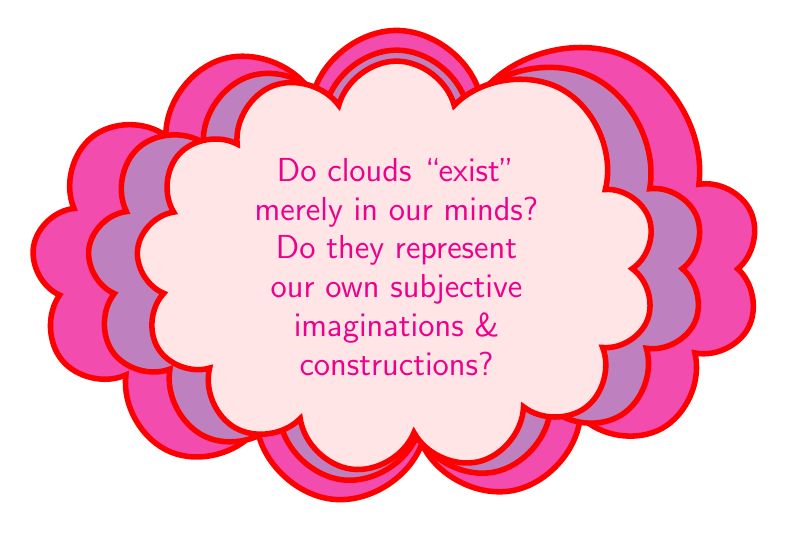
\begin{tikzpicture}  [scale=0.25,font=\large\sffamily]

\tikzstyle{every path}=[line width=2pt]
\node[cloud, cloud puffs=12.7, cloud ignores aspect, minimum width=7cm, minimum height=6cm, align=center, draw] (cloud) [color=red,fill=magenta!70]  at (0cm, 0cm) {{\color{orange}your own imagination \& construction}};
\node[cloud, cloud puffs=12.7, cloud ignores aspect, minimum width=6cm, minimum height=5.5cm, align=center, draw, text width=5cm] (cloud) [color=red,fill=violet!50]  at (0cm, 0cm)
{{\color{magenta}Do clouds ``exist'' merely in our minds? Do they represent our own subjective imaginations \& constructions?}};
\node[cloud, cloud puffs=12.7, cloud ignores aspect, minimum width=5cm, minimum height=4cm, align=center, draw, text width=4cm] (cloud) [color=red,fill=red!10]  at (0cm, 0cm)
{{\color{magenta}Do clouds ``exist'' merely in our minds? Do they represent our own subjective imaginations \& constructions?}};


\end{tikzpicture}
\end{center}


 }

\begin{frame}[fragile]{Logic/cloud does not determine the probability}


As long as there is a separating set of two-valued states
(Kochen-Specker, Theorem 0, DOI: 10.1512/iumj.1968.17.17004)
there quasi-classical analogies:
partition logics/Wright's generalized urn models/automaton logics; with classical probabilities
(convex combinations of 2-valued states):  KS arXiv:1810.10423.


\begin{center}
\begin{tabular}{cc}
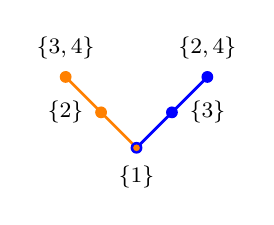
\begin{tikzpicture}  [scale=0.15]

\newdimen\ms
\ms=0.05cm

\tikzstyle{every path}=[line width=1pt]

\tikzstyle{c3}=[circle,inner sep={\ms/8},minimum size=3*\ms]
\tikzstyle{c2}=[circle,inner sep={\ms/8},minimum size=1.7*\ms]
\tikzstyle{c1}=[circle,inner sep={\ms/8},minimum size=0.8*\ms]

% Radius of regular polygons
\newdimen\R
\R=6cm     % outer circle

%\r= { \R * sqrt(3) }     % inner circle
%\newdimen\r
%\r=    {\R * sqrt(3)/2}       % inner circle

%\newdimen\K
%\K=3cm

% Define positions of all observables
\path
  (0,6 ) coordinate(1)
  (3,3    ) coordinate(2)
  (6,0 ) coordinate(3)
  (9,3) coordinate(4)
  (12,6  ) coordinate(5)
;

% draw contexts

\draw [color=orange] (1) -- (2) -- (3);
\draw [color=blue] (3) -- (4) -- (5);


%
%%
%% draw atoms
%%
%
\draw (1) coordinate[c3,fill=orange,label={above:\footnotesize $\{3,4\}$}];   %
%
\draw (2) coordinate[c3,fill=orange,label={left:\footnotesize $\{2\}$}];    %
%
\draw (3) coordinate[c3,fill=blue,label={below:\footnotesize $\{1\}$}]; %
\draw (3) coordinate[c2,fill=orange];  %
%
\draw (4) coordinate[c3,fill=blue,label={right:\footnotesize $\{3\}$}];  %
%
\draw (5) coordinate[c3,fill=blue,label={above:\footnotesize $\{2,4\}$}];  %
%
%

\end{tikzpicture}
&
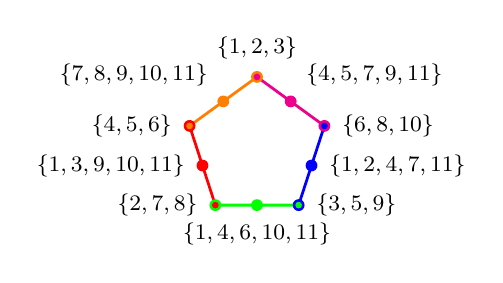
\begin{tikzpicture}  [scale=0.15]

\newdimen\ms
\ms=0.05cm

\tikzstyle{every path}=[line width=1pt]

\tikzstyle{c3}=[circle,inner sep={\ms/8},minimum size=3*\ms]
\tikzstyle{c2}=[circle,inner sep={\ms/8},minimum size=1.7*\ms]
\tikzstyle{c1}=[circle,inner sep={\ms/8},minimum size=0.8*\ms]

% Radius of regular polygons
\newdimen\R
\R=6cm     % outer circle

%\r= { \R * sqrt(3) }     % inner circle
%\newdimen\r
%\r=    {\R * sqrt(3)/2}       % inner circle

%\newdimen\K
%\K=3cm

% Define positions of all observables
\path
  ({90 + 0 * 360 /5}:\R      ) coordinate(1)
  ({90 + 36 + 0 * 360 /5}:{\R * sqrt((25+10*sqrt(5))/(50+10*sqrt(5)))}      ) coordinate(2)
  ({90 + 1 * 360 /5}:\R   ) coordinate(3)
  ({90 + 36 + 1 * 360 /5}:{\R * sqrt((25+10*sqrt(5))/(50+10*sqrt(5)))}   ) coordinate(4)
  ({90 + 2 * 360 /5}:\R  ) coordinate(5)
  ({90 + 36 + 2 * 360 /5}:{\R * sqrt((25+10*sqrt(5))/(50+10*sqrt(5)))}  ) coordinate(6)
  ({90 + 3 * 360 /5}:\R  ) coordinate(7)
  ({90 + 36 + 3 * 360 /5}:{\R * sqrt((25+10*sqrt(5))/(50+10*sqrt(5)))}  ) coordinate(8)
  ({90 + 4 * 360 /5}:\R     ) coordinate(9)
  ({90 + 36 + 4 * 360 /5}:{\R * sqrt((25+10*sqrt(5))/(50+10*sqrt(5)))}     ) coordinate(10)
;

% draw contexts

\draw [color=orange] (1) -- (2) -- (3);
\draw [color=red] (3) -- (4) -- (5);
\draw [color=green] (5) -- (6) -- (7);
\draw [color=blue] (7) -- (8) -- (9);
\draw [color=magenta] (9) -- (10) -- (1);    %


%
%%
%% draw atoms
%%
%
\draw (1) coordinate[c3,fill=orange,label=90:{\footnotesize $\{ 1,2,3\} $}];   %
\draw (1) coordinate[c2,fill=magenta];  %
%
\draw (2) coordinate[c3,fill=orange,label={above left:\footnotesize $\{ 7,8,9,10,11\}$}];    %
%
\draw (3) coordinate[c3,fill=red,label={left:\footnotesize $\{ 4,5,6\} $}]; %
\draw (3) coordinate[c2,fill=orange];  %
%
\draw (4) coordinate[c3,fill=red,label={left:\footnotesize $\{ 1,3,9,10,11\}$}];  %
%
\draw (5) coordinate[c3,fill=green,label={left:\footnotesize $\{ 2,7,8\} $}];  %
\draw (5) coordinate[c2,fill=red];  %
%
\draw (6) coordinate[c3,fill=green,label={below:\footnotesize $\{ 1,4,6,10,11\} $}];
%
\draw (7) coordinate[c3,fill=blue,label={right:\footnotesize $\{ 3,5,9\}$}];  %
\draw (7) coordinate[c2,fill=green];  %
%
\draw (8) coordinate[c3,fill=blue,label={right:\footnotesize $\{ 1,2,4,7,11\}$}];  %
%
\draw (9) coordinate[c3,fill=magenta,label={right:\footnotesize $\{ 6,8,10\}$}];
\draw (9) coordinate[c2,fill=blue];  %
%
\draw (10) coordinate[c3,fill=magenta,label={above right:\footnotesize $\{ 4,5,7,9,11\}$}];  %
%
%
\end{tikzpicture}
\\
(a)&(b)
\end{tabular}
\end{center}


Quantum realization in terms of the faithful orthogonal representation (Lov\'asz, Saks and Schrijver DOI 10.1016/0024-3795(89)90475-8)
and the Theta-body (Gr{\"o}tschel,Lov{\'a}sz and Schrijver DOI: 10.1016/0095-8956(86)90087-0)


\end{frame}

\begin{frame}[fragile]{Anecdotal examples of ``exotic'' probability measures satisfying Kolmogorovian classical probabilitie on local contexts}



\begin{itemize}

\item Wright's (1978) dispersionless measure on the pentagon (or cyclic arrangements of odd contexts $\ge 3$

\item  Godsil and J. Zaks (1988) Coloring the sphere (arXiv:1201.0486) stimulates Meyer's ``Nullification'' of the Kochen-Specker theorem (DOI: 10.1103/PhysRevLett.83.3751):
use unit vectors with rational coefficients: dense but discontinuous (Havlicek, Krenn, Summhammer and KS, DOI: 10.1088/0305-4470/34/14/312 )



\end{itemize}

\end{frame}


\frame{

\centerline{\huge {\color{yellow} Thank you for your attention!}}

\begin{center}\color{orange}
$\widetilde{\qquad \qquad }$
$\widetilde{\qquad \qquad}$
$\widetilde{\qquad \qquad }$
\end{center}
 }
 \end{document}








 \frame{
 \frametitle{}

 }


